\usepackage[utf8]{inputenc}
\usepackage[round]{natbib}
%Information to be included in the title page:
\title{The Biogeochemical Model Database}
\subtitle{Python packages for \alert{model intercomparison}}
\author{Markus Müller}
%\institute{Overleaf}
%\date{11-16-2021}
\date{\today}
\usepackage{tikz}
\usetikzlibrary{positioning}
\begin{document}
\titlepage
\begin{frame}
\frametitle{Overview}
\tableofcontents
\end{frame}
\section{\texttt{bgc\_md2} Screenshots}
\subsection{Views}
\begin{frame}
\frametitle{Jupyterwidget for a subset of models \texttt{bgc\_md2} }
	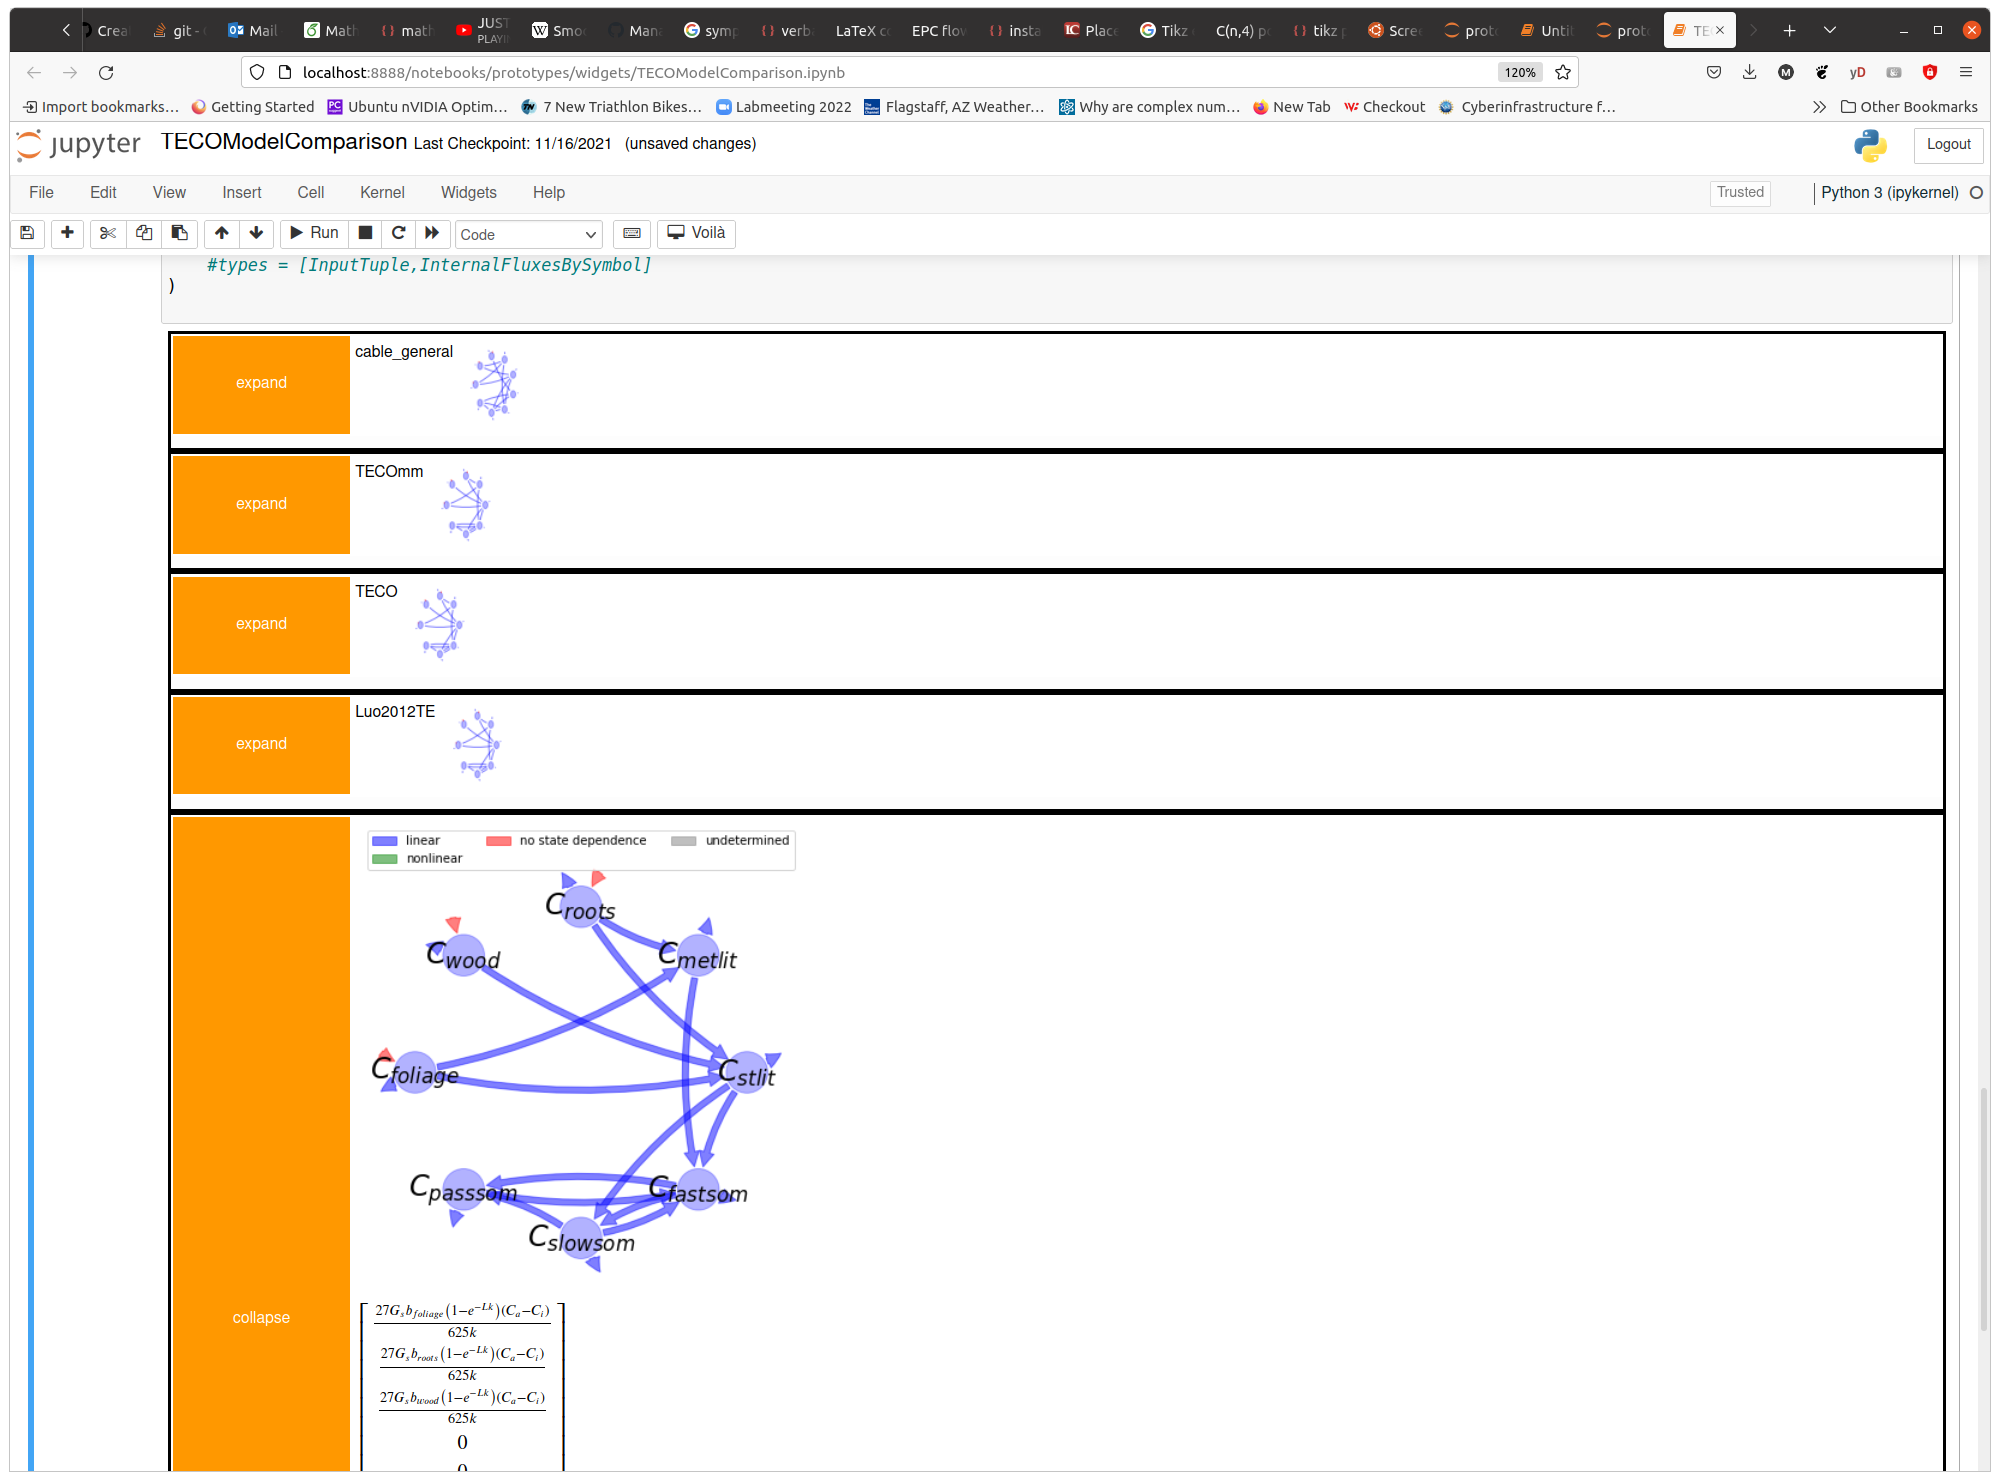
\includegraphics[width=\textwidth]{ModelTable.png}
\note{
	\begin{enumerate}
	\item
	bgc\_md2 is an open source python package availabe on GitHub, developed at the Max-Planck-Institut for BioGeoChemistry in Jena and more recently  in Yiqi Luo's Ecolab at NAU in Flagstaff in Cornell and now in the Research Center Juelich
	\item
	A set of libraries that can be used in other python scripts or interactively (jupyter or IPython )
	The picture shows a jupiter widget showing a table of models. The orange buttons can be clicked to 
	expand or collape a more detailed view of the particular model.
	\item
	$>$ 30 published vegetation, soil or ecosystems models in a format that
	for symbolic and numeric computations
	\item
	A set of special datatypes that describe components of the models and functions that operate on these datatypes
	\item 
	A userinterface that uses a graph library to compute what is computable and can be used for comparisons.
	\end{enumerate}
}
\end{frame}

\subsection{Single Model Inspection}
\begin{frame}
	\frametitle{Analysis with symbolic tools \dots}
	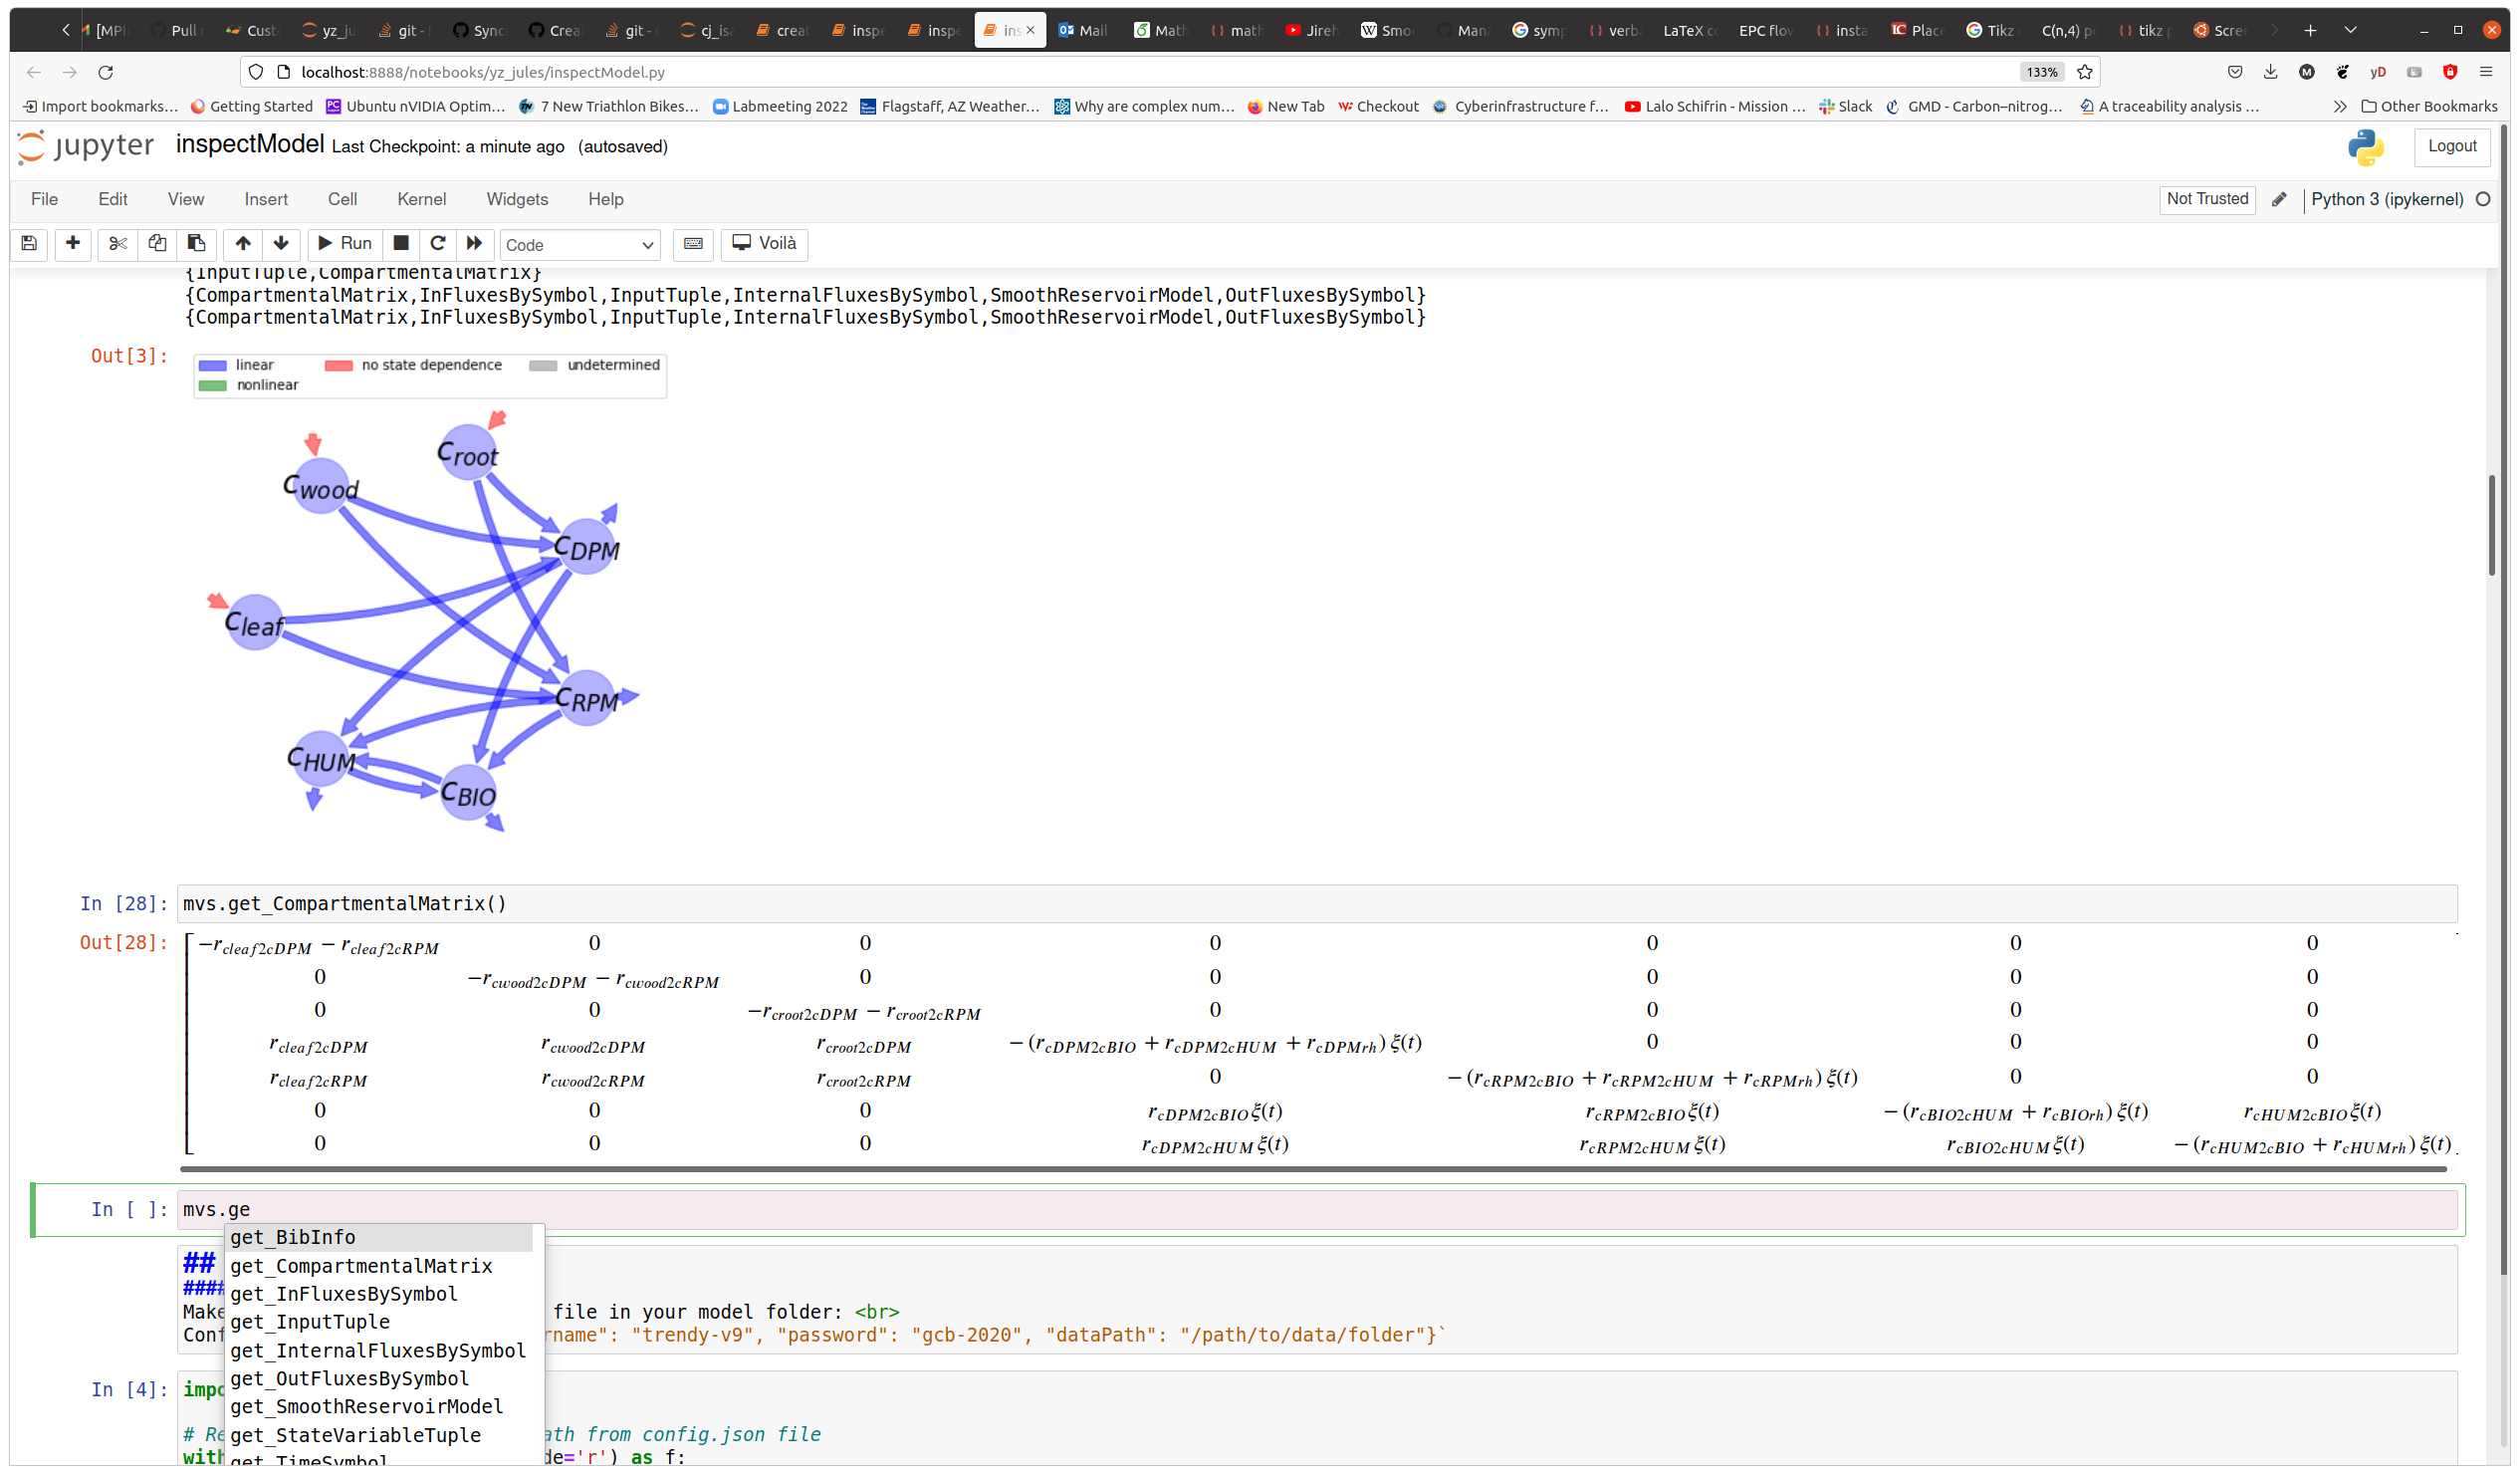
\includegraphics[width=\textwidth]{mvsTabScreen.png}
	\note{
	\begin{enumerate}
	\item 
	the structure (graph both in the mathematical and visual sense) can be derived from the symbolic description
	\item other properties are flux equations the compartmental matrix

	\end{enumerate}
	}
\end{frame}

\begin{frame}
	\frametitle{\dots or numerically }
	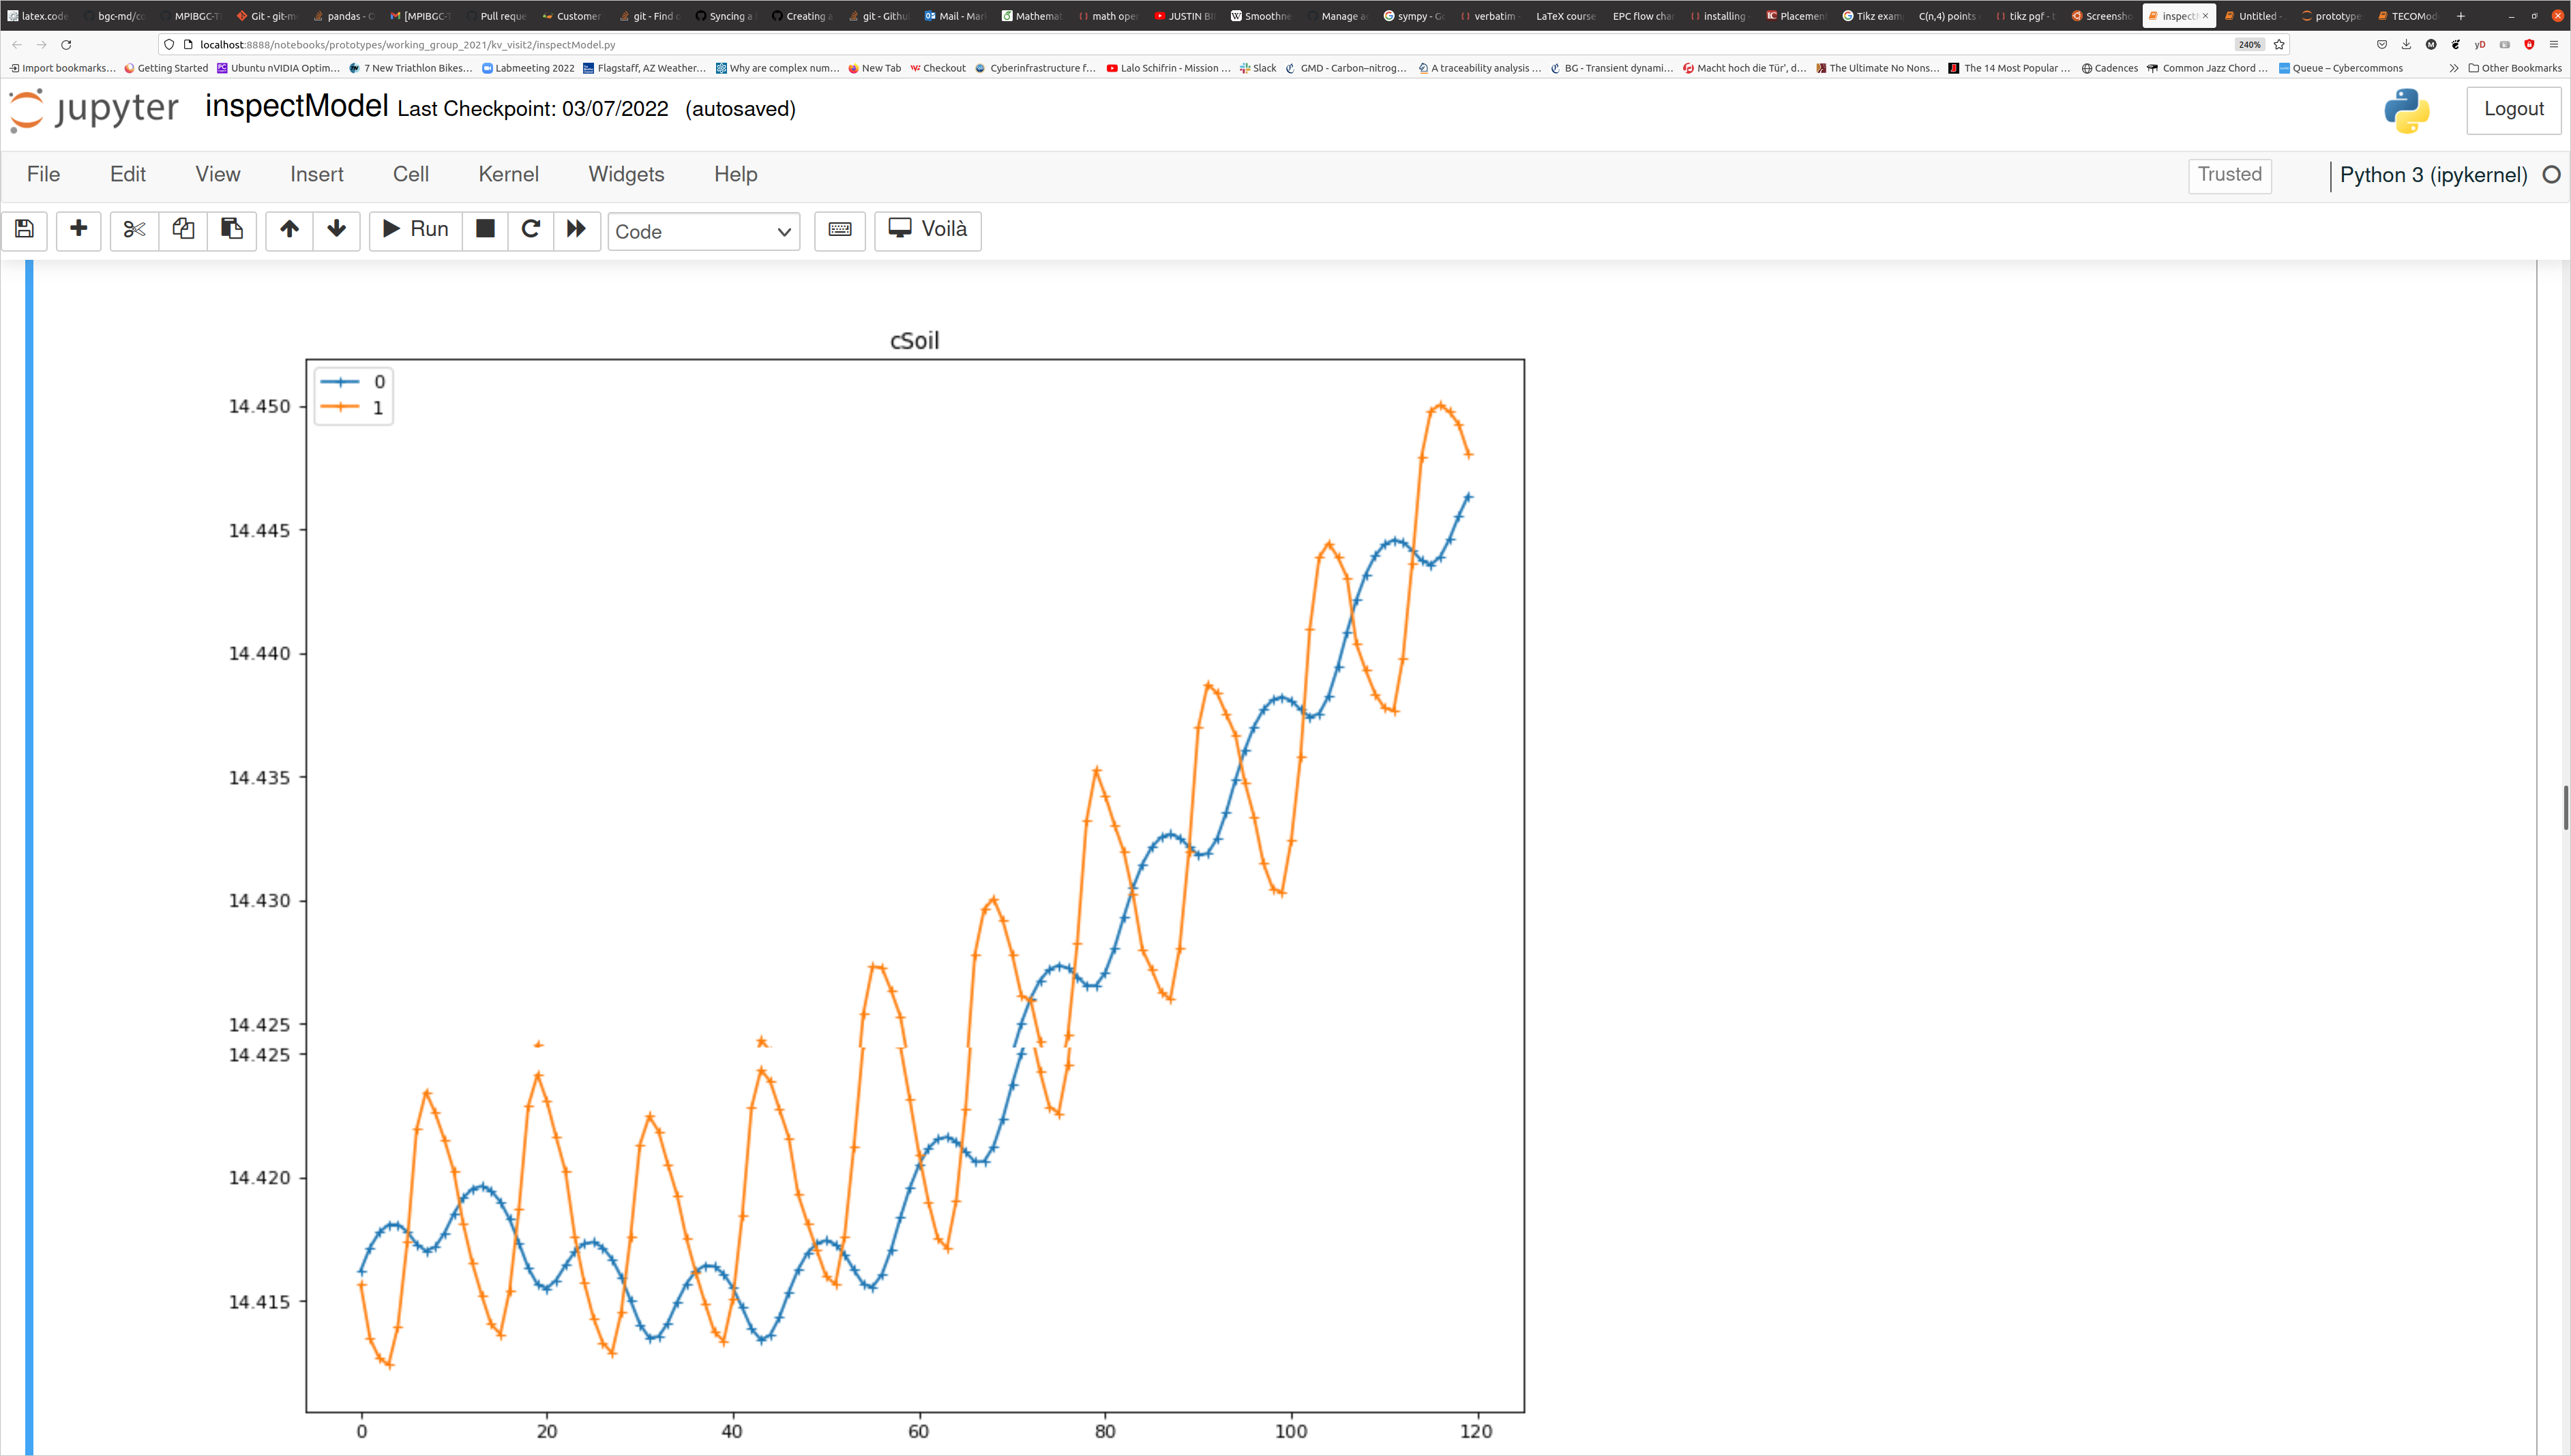
\includegraphics[width=\textwidth]{DataAssimilation.png}
	\note{
	\begin{enumerate}
	\item 
	the symbolic model description can be parameterized and transformed into a numeric model
	\item The picture shows the data assimilation result for the above model using trendy data.

	\end{enumerate}
	}
\end{frame}

%\begin{frame}
%	\frametitle{Diagnostic Variables implemented once, available for all models}
%	\begin{figure}
%	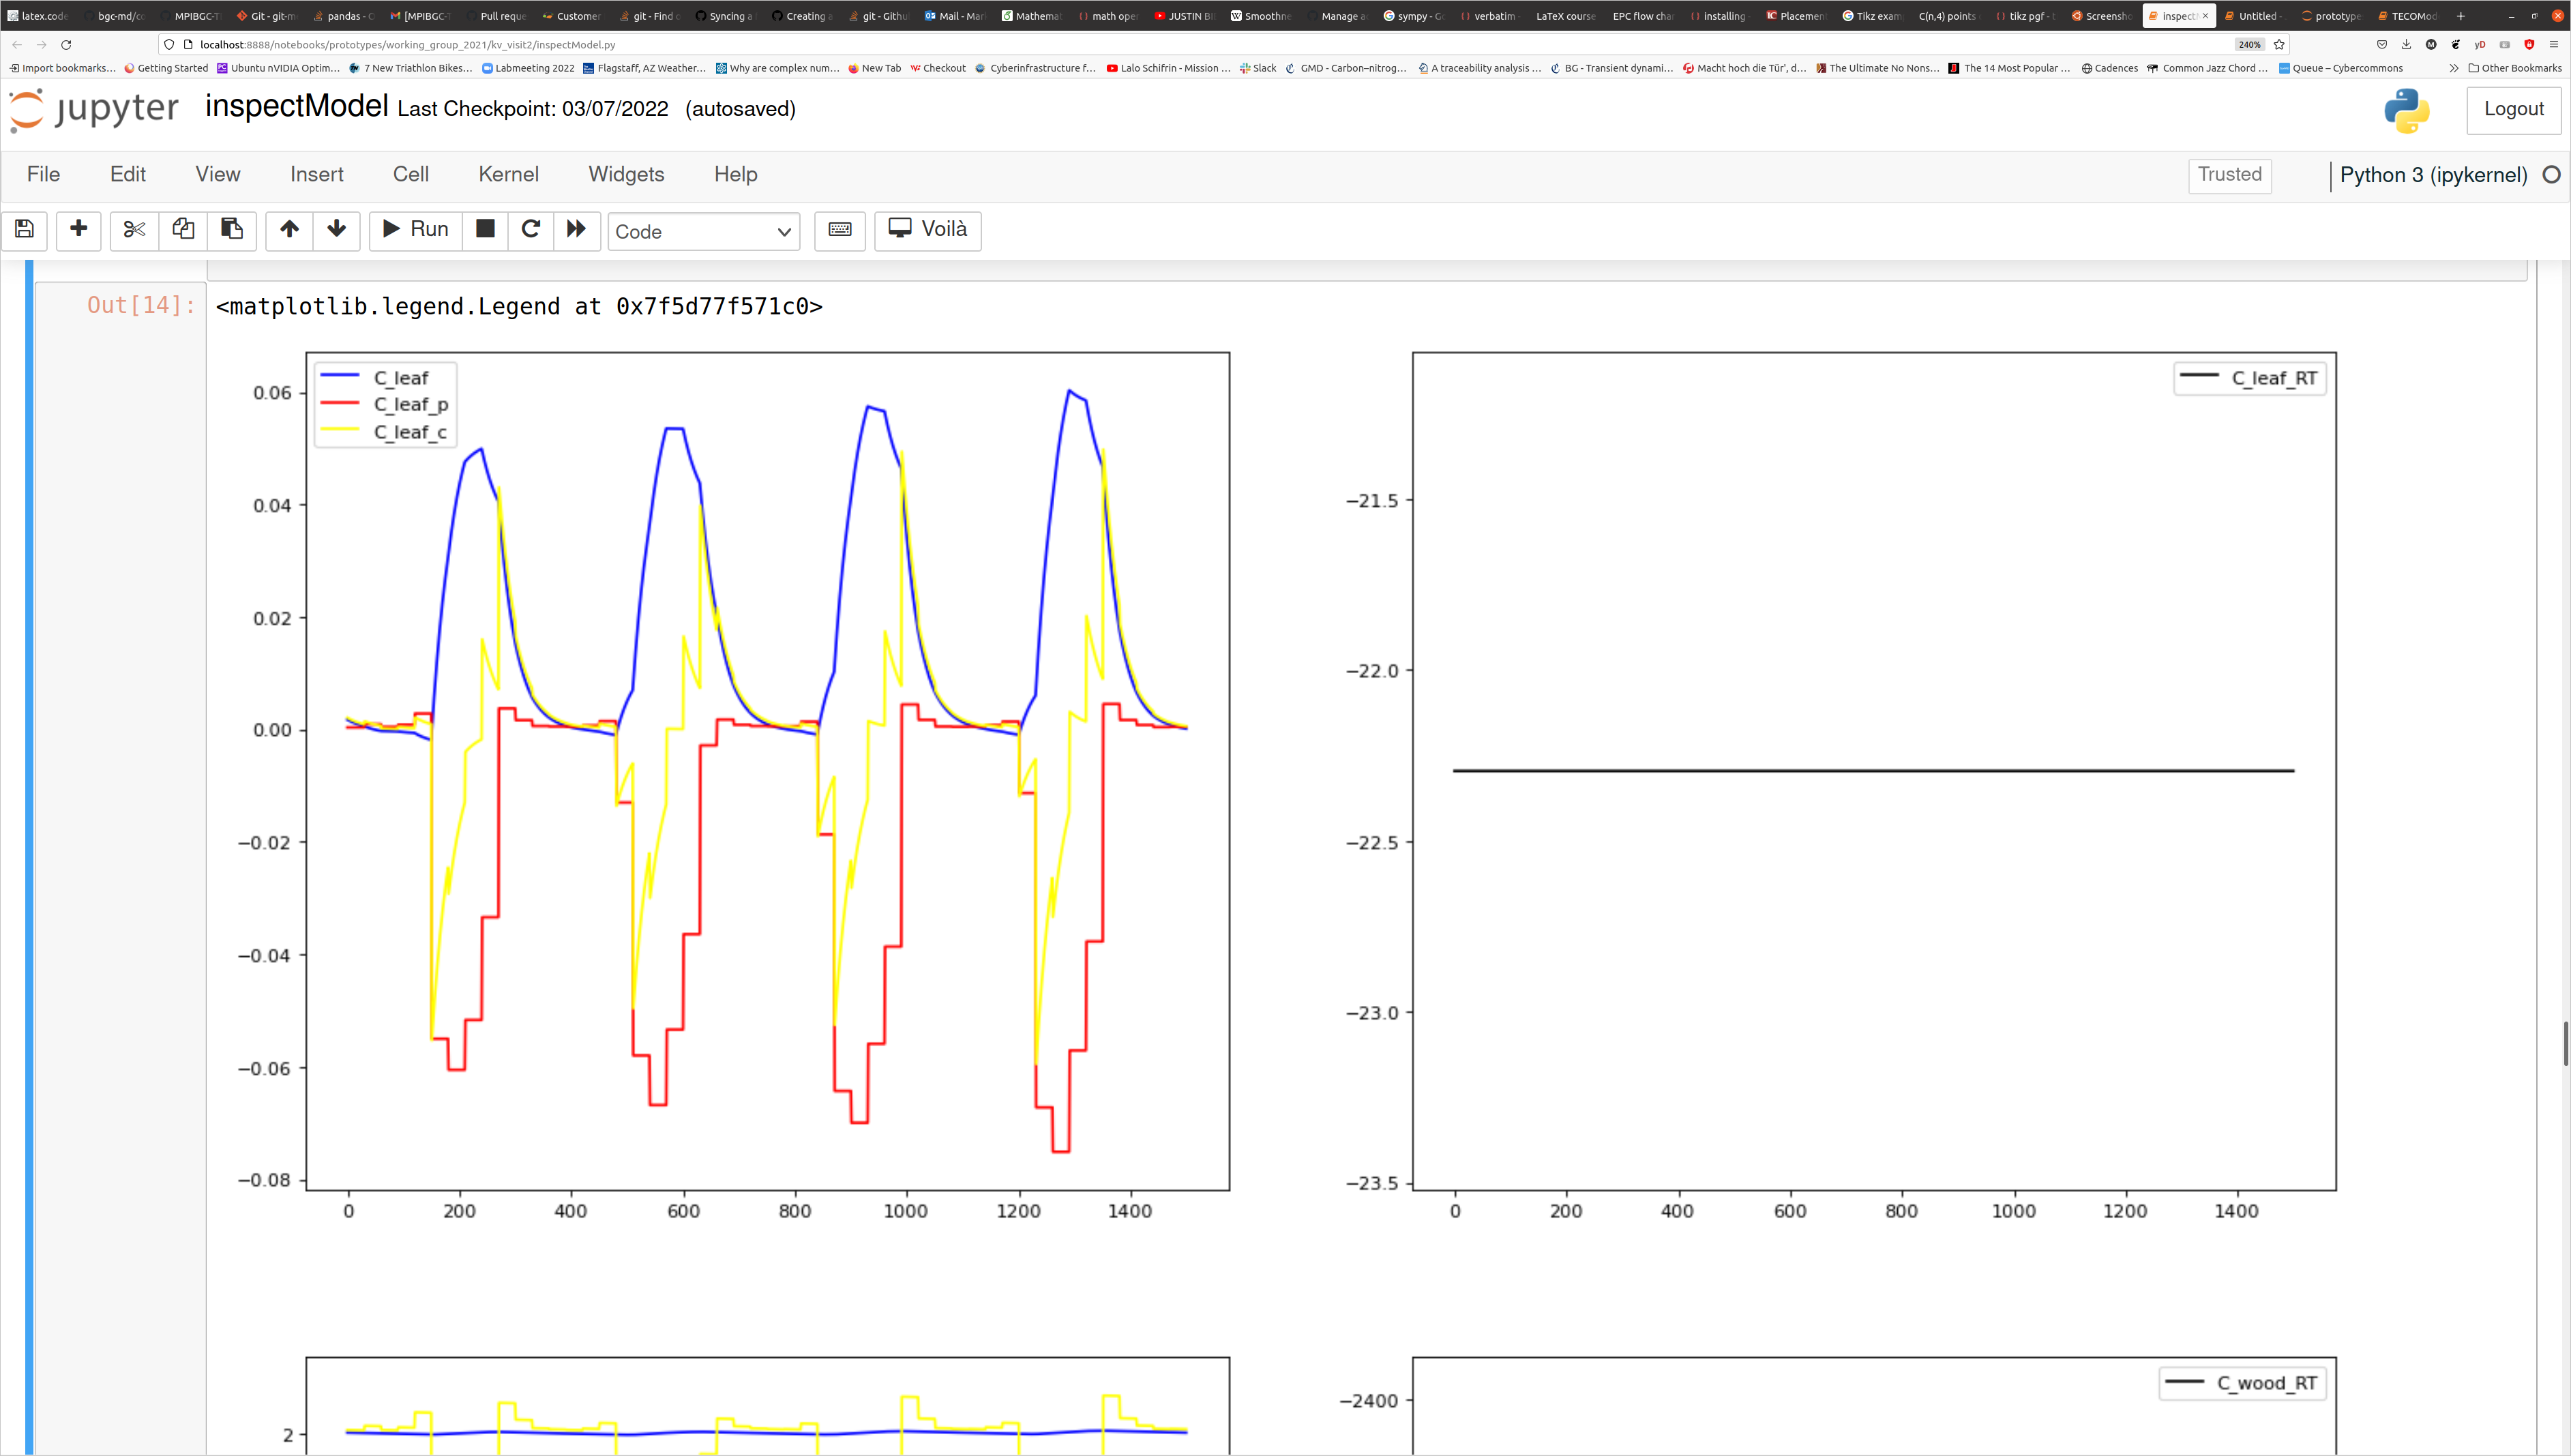
\includegraphics[width=\textwidth]{TracebilityAnalysis.png}
%	\caption{pool content + Tracebility Analysis: carbon storage potential , carbon storage capacity and residence time}
%	\end{figure}
%	\note{
%	\begin{enumerate}
%	\item 
%	Diagnostic Variables can be computed for any model  
%	\item The picture shows the Leaf pool
%
%	\end{enumerate}
%	}
%\end{frame}

\section{User Interface and Queries}
\subsection{Invisible Graphs}
\begin{frame}
  \frametitle{Userinterface using computability graphs}
  \begin{figure}
  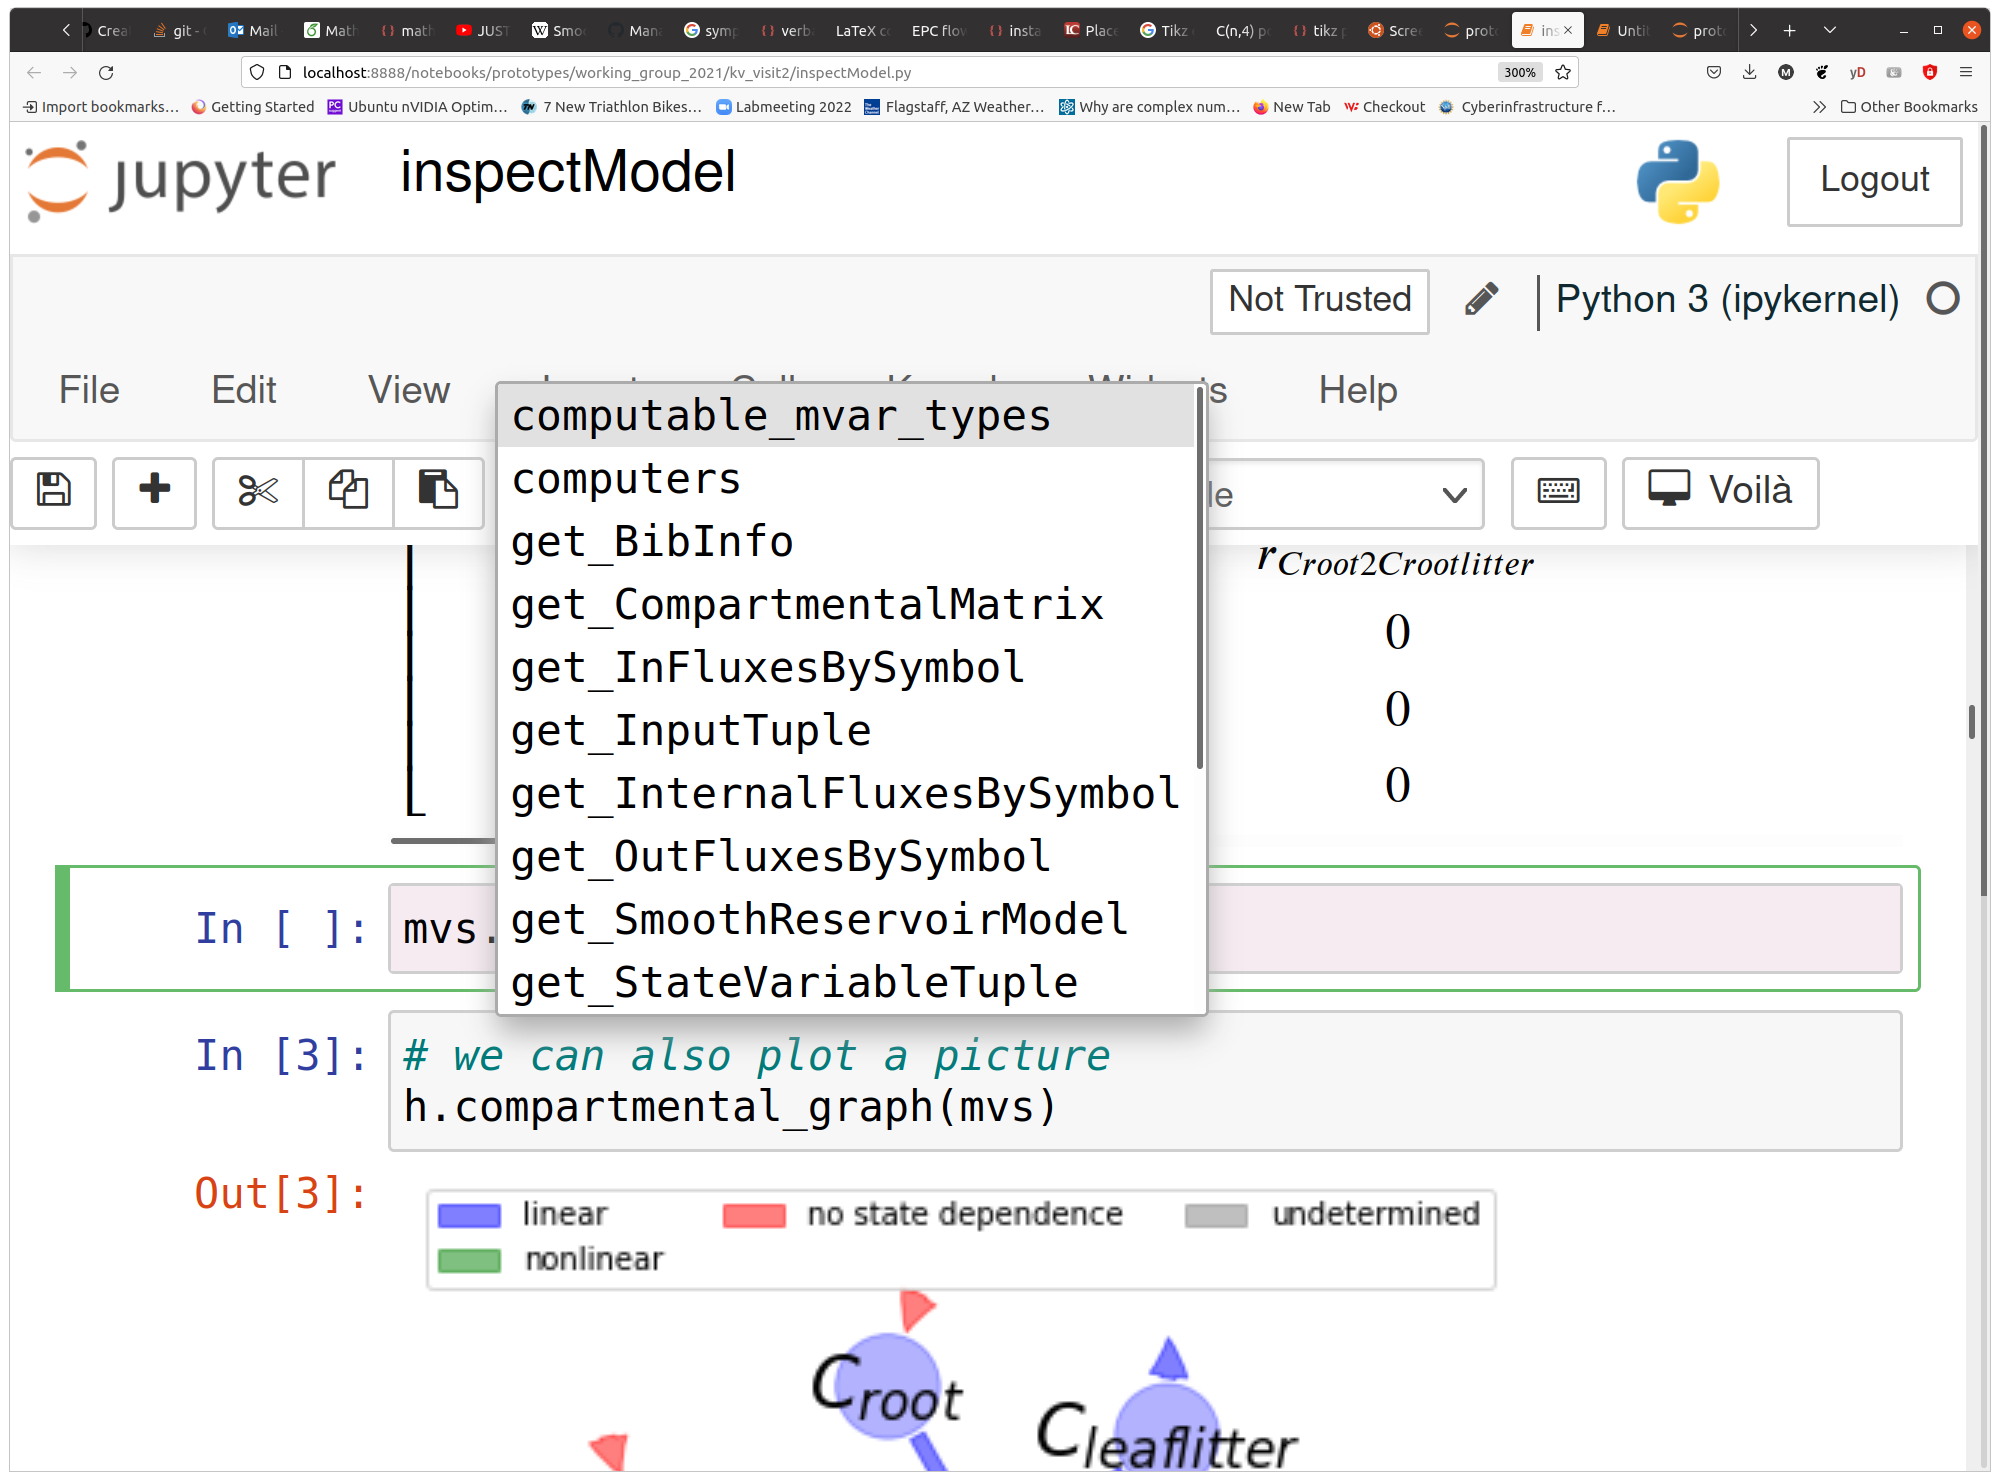
\includegraphics[height=0.8\textheight]{mvsTabScreenBig.png}
  \caption{Suggested methods automatically created by a graph library}
  \end{figure}
  \note{
  \begin{tiny}
    \begin{enumerate}
    \item
    The figure shows IPythons options for callable methods on a variable called \texttt{mvs} 
    \item
    This is standard for mehtods of a python object. 
    In this case the methods are automatically created and added by a graphalgorithm that computes 
    which variables can be computed form the set of provided model properties.
    \item 
    This has far reaching consequences.
    Models can be compared with respect to all variables in the "convex hull under computability', 
    with respect to all \emph{computable variables} not just the ones provided in the data base record.
    \item
    As an example the matrix formulation of models A and B  can be compared even if neither A nor B defines
    the matrix as long as it can be computed from other variable (in this case the internal and outfluxes and an ordering of the statevariables)
    \item
    An obvious consequence is that the information about a model can be provided in different ways.
    There is no need to force the user into a rigid record format.
    Another consequence is that records do not have to be complete. The framework accepts all information
    about a model and (computes what it can do with it).
    \item
    The set of computable properties can be used to query the database (e.g. which models have a vegetation part)
    \dots
    \end{enumerate}
  \end{tiny}
  }
\end{frame}

\subsection{Making them Visible }
\begin{frame}
\frametitle{Finding what's missing}
\begin{columns}
  \begin{column}{0.3\textwidth}
  given a set of functions:\\
        a(i), b(c,d), b(e,f), c(b),
        d(b), d(g,h),
        e(b),
        f(b)
  and the target variable {\color{red}B}
  e.g. \texttt{CompartmentalMatrix},
  The algorithm computes all possible combinations
  and paths from which {\color{red}B} can be computed.
  \end{column}
  \begin{column}{0.7\textwidth}
      \begin{center}
      \begin{figure}
  	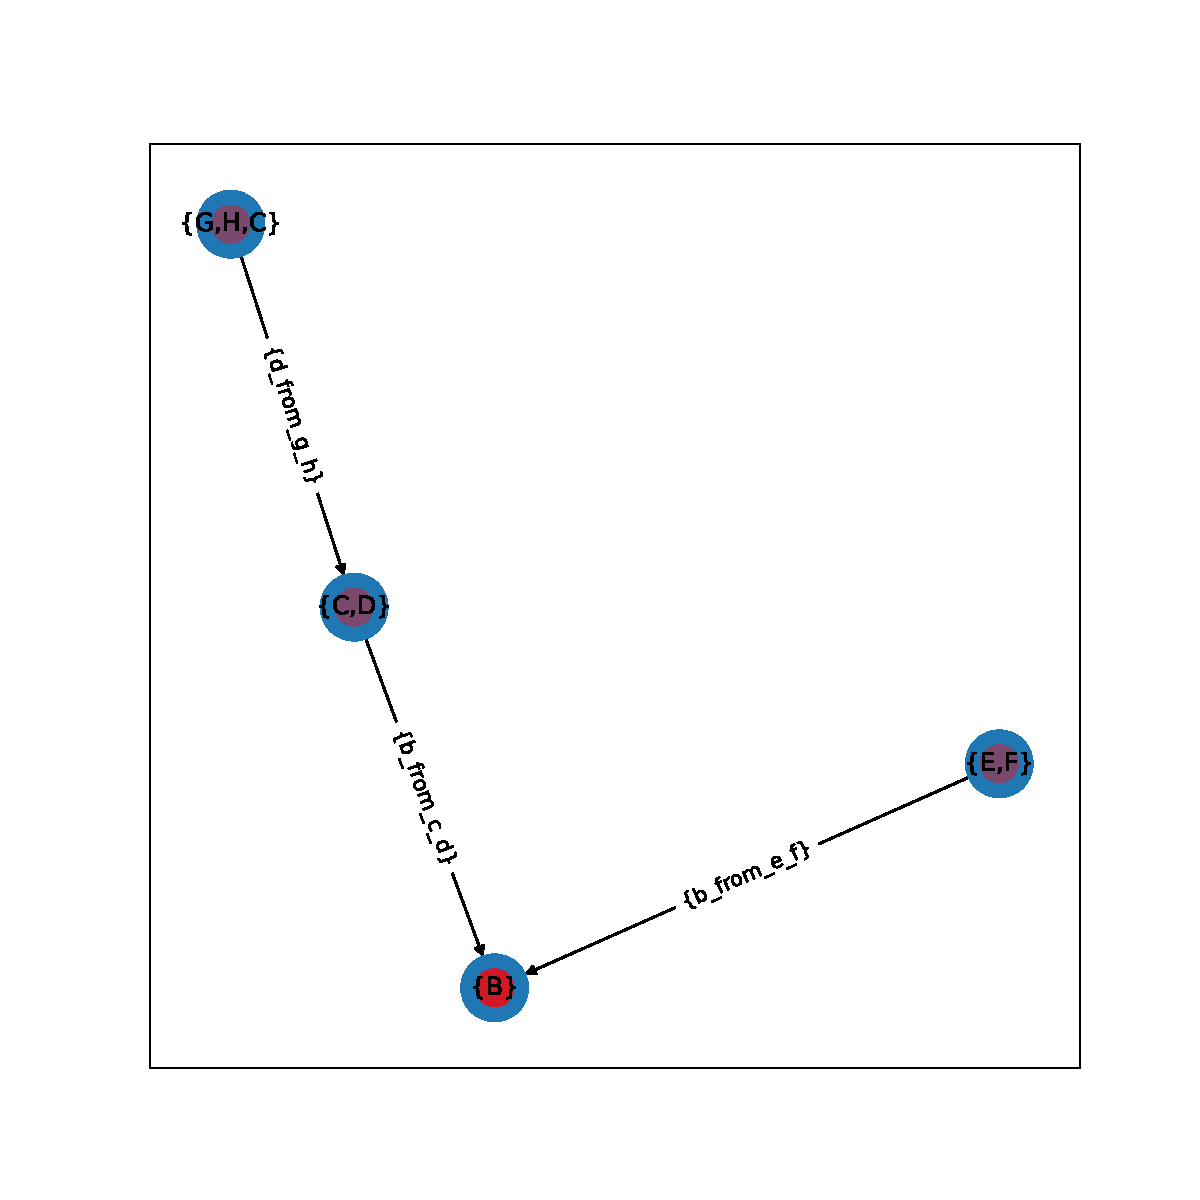
\includegraphics[width=\textwidth]{StartNodes.pdf}
	%\caption{The computability Graph for variable B (e.g. \texttt{CompartmentalMatrix}}
      \end{figure}
       \end{center}
  \end{column}
\end{columns}
  \note{
    \begin{enumerate}
    \item
    It is not only possible to compute what can be computed from a given model description,
    It is also possible to do the opposite and ask the algorithm what missing information has to be 
    provided to compute a target property of a  model.
    \item
    The algorithm finds a path (a combination of functions that can be applied recursively) and automatically computes intermediate results. 
    \end{enumerate}
  }
\end{frame}

\section{Structure}
\subsection{Classes \emph{and} Functions}
\begin{frame}
\frametitle{Internal Structure of \texttt{bgc\_md2}}
\begin{tikzpicture}[sibling distance=12em,
  every node/.style = {shape=rectangle, rounded corners,
    draw, align=center,
    top color=white, bottom color=blue!20}]]
  \tikzstyle{level 1}=[sibling distance=14em]
  \tikzstyle{level 2}=[sibling distance=5em]
  \tikzstyle{level 3}=[sibling distance=3em]
  \tikzstyle{level 4}=[sibling distance=1.75em]
    \node {% <- this 'right of' is inherited; how to avoid?
    \begin{tikzpicture}[anchor=center]
      \node {\texttt{bgc\_md2}
      %\draw (0,0) -- (0,1);
      %\node[fill] at (0,.5) {};
      } 
      child{ node {models}
	 child{ node{rothC}
	    child{node {Fluxes}}
	    child{node {Pools}}
	    child{node {\dots}}
	}
      	child{ node {Wang}
	%    child{node {Fluxes}}
	%    child{node {Pools}}
	%    child{node {\dots}}
	}
      	child{ node {\dots}}
      }
      child{ node {computers}
	 child{node {Matrix(Fluxes)}}
	 %child{node {Fluxes(Matrix,Pools)}}
	 child{node {\dots}}
      };
    \end{tikzpicture}
    };
\end{tikzpicture}
\note{
  \begin{enumerate}
    \item
    \texttt{bgc\_md2} is not just a collection of models, described as sets of varible of special type like fluxes or matrice, but also 
    a collection of functions whose arguments and return values have these types.
    These functions are here called \texttt{computers} and use python type annotations.
    The computability graph used in the user interface and queries is derived from the 
    annotations of a set of functions.
    The set of properties (defined by the types) is growing as well as the functions connecting them.
  \end{enumerate}
}
\end{frame}

\subsection{A Record}
\begin{frame}
\frametitle{Database records are python modules}
  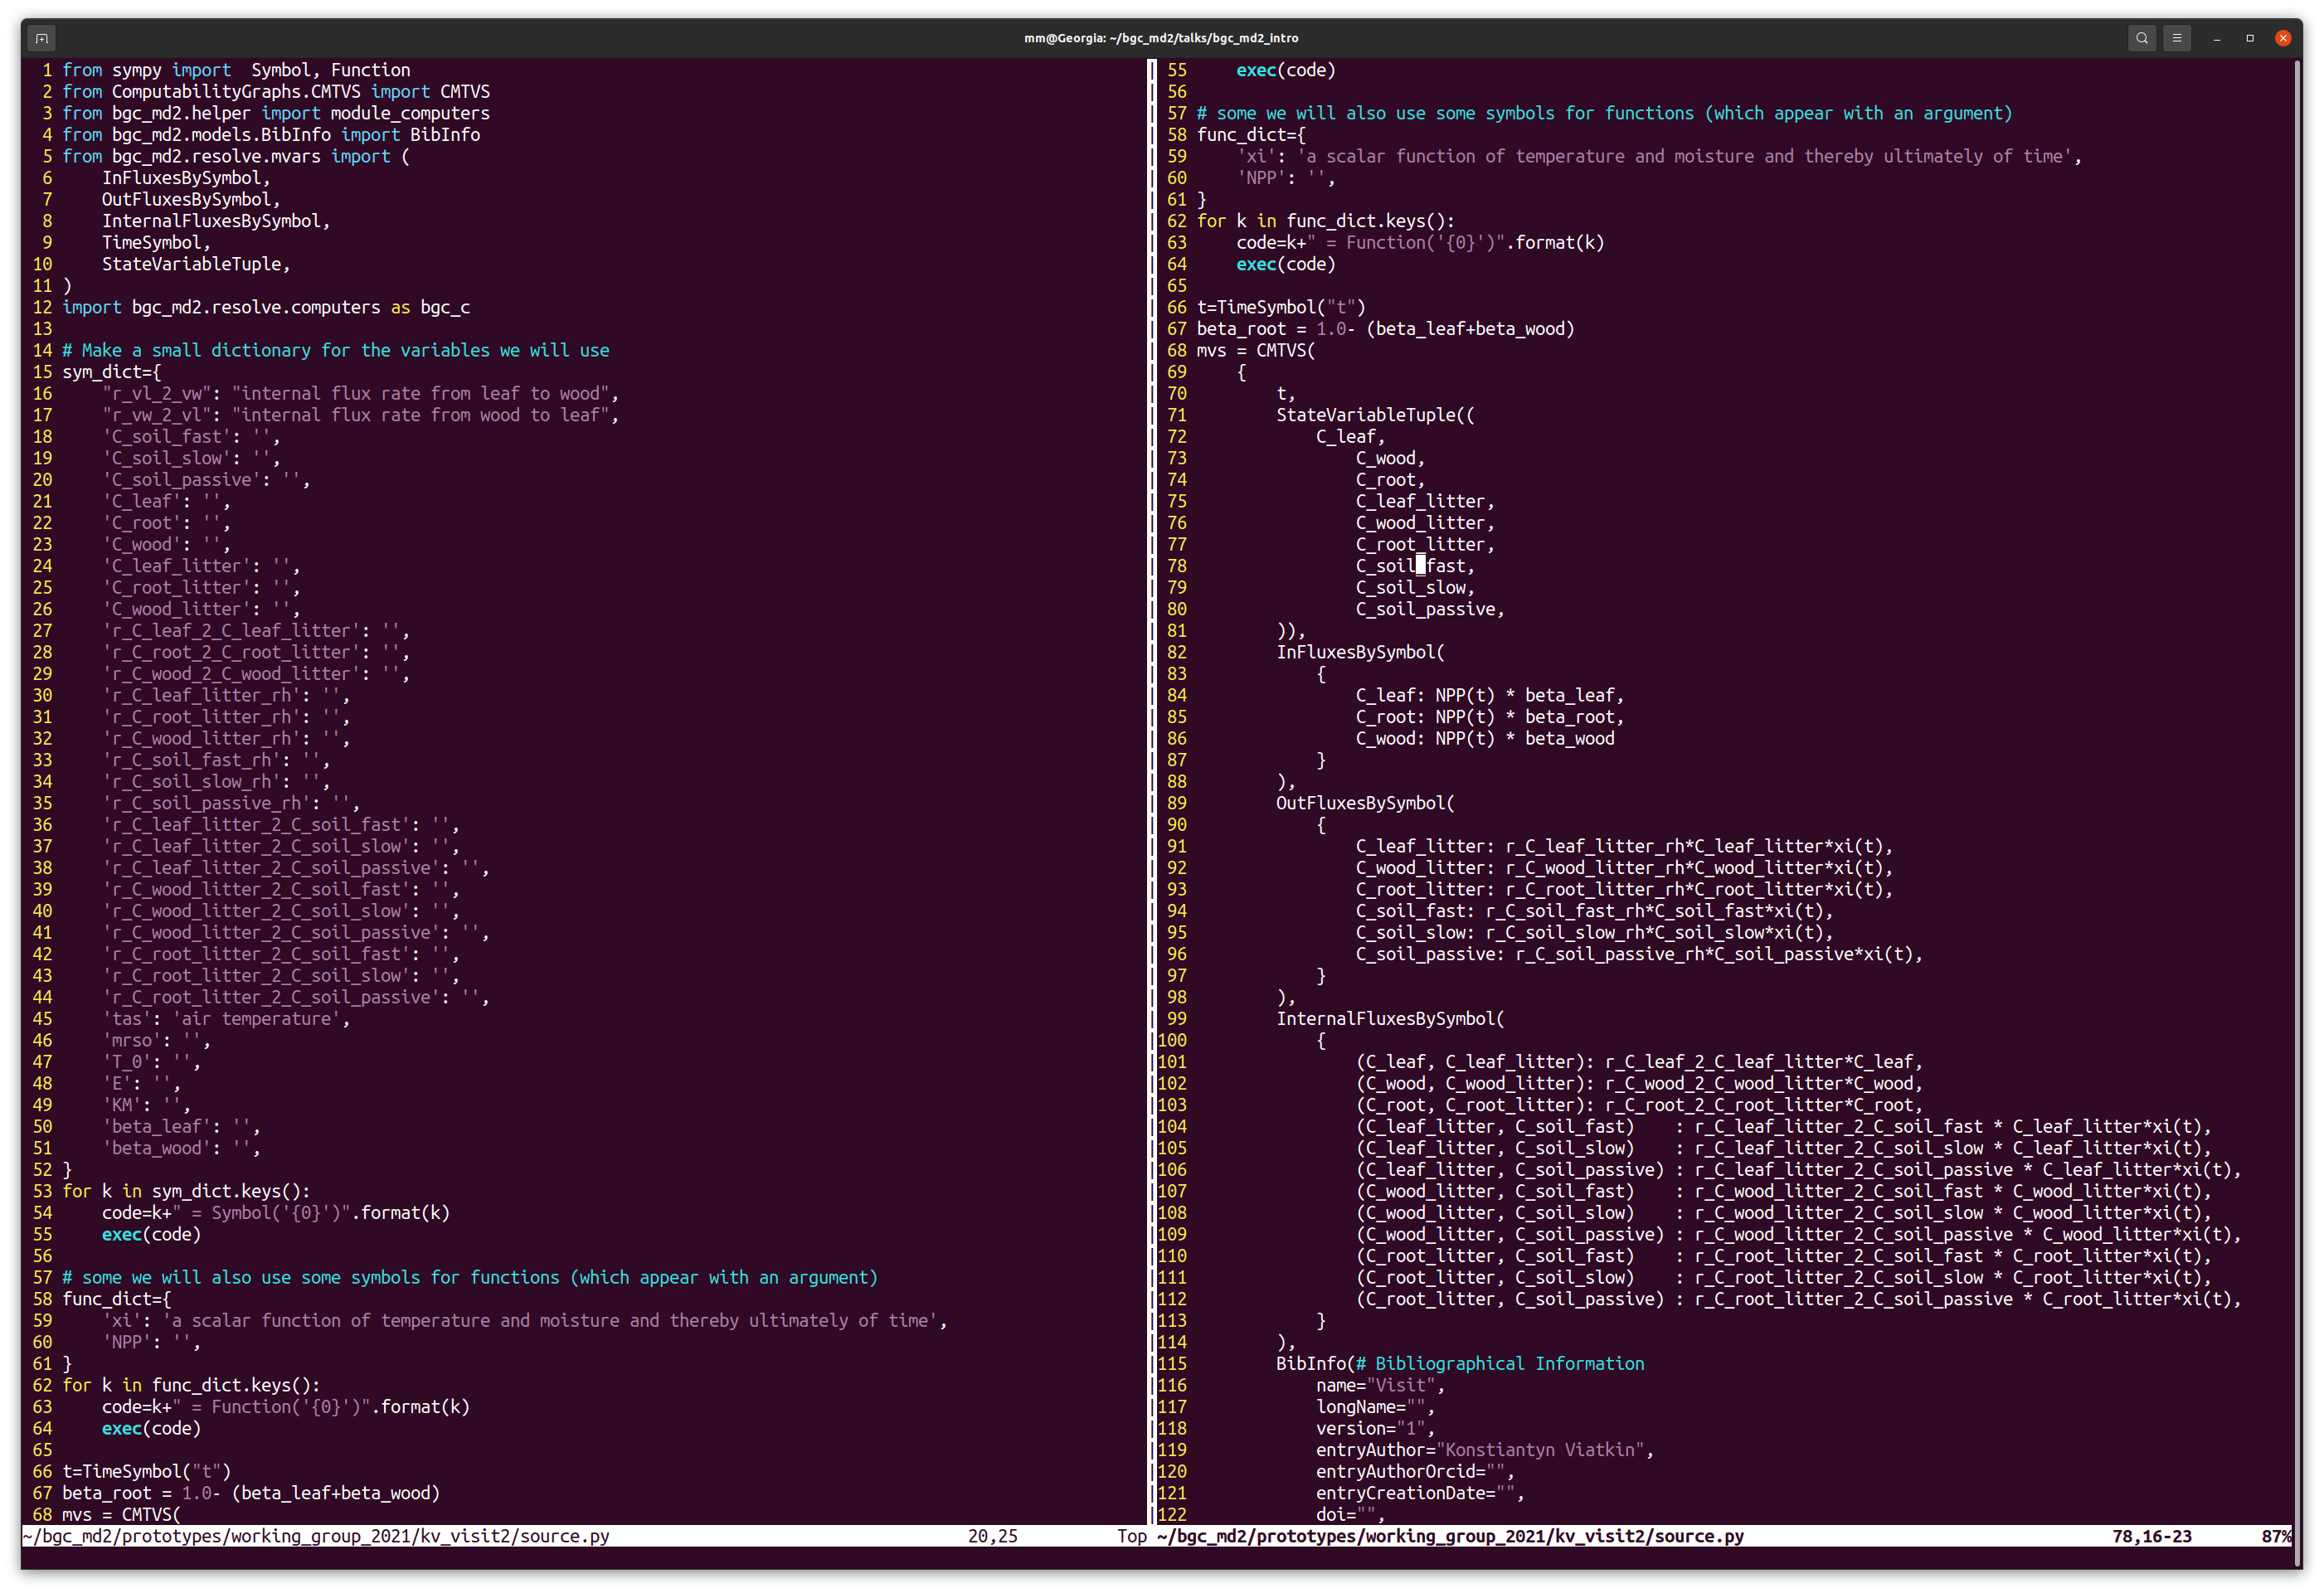
\includegraphics[width=\textwidth]{source.py.png}
  \note{
  \begin{enumerate}
    \item
    The picture shows the screen shot of the source code of the above model using sympy and some datatypes provided by \texttt{bgc\_md2}  .
    \item
    The entries of the database dont even have to be complete models. They are implemented in normal python and 
    have in common that they define a set of model properties and a set of functions to connect them.
    There is no special format necessary. 
    The creation of the symbolic formulation can be automated by all means available in python.
    Extra information can but does not have to be provided.
  \end{enumerate}
}
\end{frame}

\subsection{Relation to other Python Packages}
\begin{frame}
\frametitle{Relation to other Python Packages}
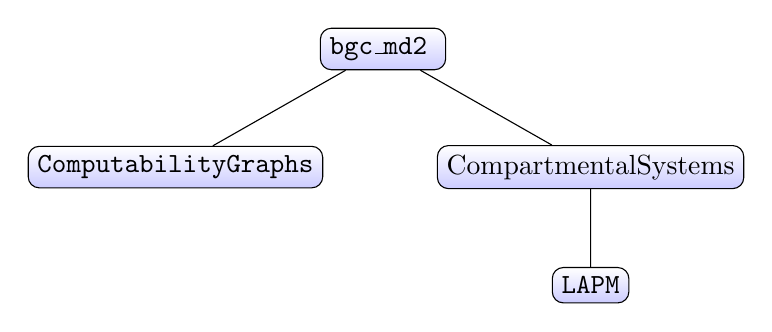
\begin{tikzpicture}[sibling distance=15em,
  every node/.style = {shape=rectangle, rounded corners,
    draw, align=center,
    top color=white, bottom color=blue!20}]]
    \node {
    	\texttt{bgc\_md2}
    }
    child { node {\texttt{ComputabilityGraphs}} }
	child { node[sibling distance=5em]{CompartmentalSystems}
	child { node (LAPM){\texttt{LAPM}} }
	%child [level distance=10em]{ node [style ={top color=white,bottom color=black!10}](SymPy){\texttt{SymPy}} }
	%child [level distance=10em]{ node [style ={top color=white,bottom color=black!10}](SymPy){\texttt{nupy}} }
   };
	%\draw[->] (LAPM) -- (SymPy); 
\end{tikzpicture}
  \note{
  \begin{enumerate}
    \item
    The graph computation is outsourced into our package \texttt{ComputabilityGraphs} 
    \item
	    Many of the advanced diagnostic variables (age and transittime distributions) are computed using our other packages \texttt{LAPM} and \texttt{CompartmentalSystems} for which \texttt{bgc\_md2} acts as interface.
  \end{enumerate}
}
\end{frame}
\section{Non trivial diagnaostic variables}
\subsection{Transient age and transit time distributions for nonlinear nonautonomous compartmental models}
\begin{frame}
	\frametitle{Applications}
	\begin{figure}
	
\includegraphics[height=0.5\textheight]{atmosphere_nonlinear.pdf}
		\caption{age distribuition of a pool as function of time}
	\end{figure}
	\begin{thebibliography}{}
	\bibitem[Metzler, Müller, Sierra, 2018]{Metzler2018PNAS}
	Metzler, H., M{\"u}ller, M., and Sierra, C. (2018).
	\newblock Transit-time and age distributions for nonlinear time-dependent
	  compartmental systems.
	\newblock {\em Proceedings of the National Academy of Sciences}, 115:201705296.
	\end{thebibliography}
\end{frame}

\begin{frame}
\frametitle{Summary: Give me what you have and I"ll show you what I can do with it} 
  \texttt{bgc\_md} is a library providing:
  \begin{enumerate}
    \item
      Datatypes defining building blocks of models e.g.\ \texttt{CompartmentalMatrix}, \texttt{InternalFluxesBySymbol}, \dots     
    \item
      Functions operating on those properties (forming the edges of the graph where the Datatypes are nodes) 
    \item
      A user interface based on graph algorithms to  
    \begin{enumerate}
      \item
        compute the set of computable properties (e.g. the comparable criteria for a set of models, database queries ) 
      \item
        actually compute the desired properties by recursively connecting several function applications.
      \item
        show what is missing to compute a desired property.
    \end{enumerate}
    \item
    $30+$ vegetation, soil or ecosystem models for carbon and nitrogen cycling
      as reusable python modules using the building blocks in a flexible way. 
    \item 
      An interface to \emph{many  algorithms} in \texttt{CompartmentalSystems} to compute diagnostic variables
      for \emph{many models} in \texttt{bgc\_md2}.
  \end{enumerate}
\end{frame}

%%%%%%%%%%%%%%%%%%%%%%%%%%%%%%%%%%%%%%%%%%%%%%%%%%%%%%%%%%%%%%%%%%%%
\section{Application to  model intercomparison}
\subsection{Goals}
%%%%%%%%%%%%%%%%%%%%%%%%%%%%%%%%%%%%
\begin{frame}
  \frametitle{We might want to know ...}
  \begin{itemize}
  \item 
   If two or more (published) models are possibly possibly { \it identical}.
   \item
   If not, if they have some things in common and which.
   \item
   How they differ.
   \item
   If one is a generalization of another.
   \item
   If there are 'normal forms' e.g. views that hide incosequential details.
   \item
   Which model fits the data better.
   \item
   What constitutes a model. (Definitions may depend on the questions.)
  \end{itemize}
\end{frame}

\begin{frame}
  \frametitle{Three Soil Models} 
  \includegraphics[height=0.3\textheight]{physIndex.pdf}
  \includegraphics[height=0.3\textheight]{dormancy_2_Monod_compartmental.pdf}
  \includegraphics[height=0.5\textheight]{dormancy_4_Monod_compartmental}
\end{frame}


\begin{frame}
\frametitle{Symbolic comparison (pools) } 

\only<1>{
  \includegraphics[width=\textwidth]{Dormancy2_metamorphosis.pdf}
}
\only<2>{
  \includegraphics[width=\textwidth]{Dormancy2_metamorphosis_2.pdf}
}
Can be done by \texttt{bgc\_md2} with a (python) dictionary for the variable names and a definition of the sets of pools that form the new superpools 
$\{ X_a, X_d \} \rightarrow X$
\end{frame}


\begin{frame}
\frametitle{Symbolic comparison (equations) } 
\begin{itemize}
  \item
  Translation of the ODE
  can also be assisted by \texttt{bgc\_md2} with  sympy. 
  \begin{align*}
  \left.
  \begin{matrix}
    \dot{X_a}=f(X_a,X_d,X_n,S,\mathbf{p}) \\
    \dot{X_d}=g(X_a,X_d,X_n,S,\mathbf{p}) \\
    \vdots \\
    X_a(t_0)={X_a}_0 \\
    X_d(t_0)={X_d}_0 \\
    \vdots \\
  \end{matrix}
  \right \} 
  \underbrace{\rightarrow}_{R=\frac{X_a}{X_a+X_d}} 
  \left \{
  \begin{matrix}
    \dot{X}=h(X,R,N,S,\mathbf{p}) \\
    \dot{R}=j(X,R,N,S,\mathbf{p}) \\
    \vdots \\
    X(t_0)={X}_0 \\
    R(t_0)={R}_0 \\
    \vdots \\
  \end{matrix}
  \right.
  \end{align*}
  %\item
  %Translation of the constraints.
  %\alert{Cannot} be done yet, because the constraints are not explicitly available in the model database. 
\end{itemize}
The constraints are an essential part of the model. (As we will see later)
\end{frame}
%
\subsection{Numeric comparison}
\begin{frame}
\frametitle{Forward simulations with given parameters (easy)} 
  \includegraphics[width=\textwidth]{Numeric1.pdf}
  Automatic unit conversion (different models have different units)
\end{frame}

\begin{frame}
\frametitle{Forward simulations with given parameters (easy) II} 
  \includegraphics[width=\textwidth]{NumericII.pdf}
 Lots of derived "diagnostic" variables, which can be computed for both models and allow comparison on a meta level.  
\end{frame}

\begin{frame}
\frametitle{Parameter estimation (hard)} 
  \includegraphics[width=\textwidth]{NumericIII.pdf}
  Hard because we have to be fair. Both models must have the same chance to hit the data.
\end{frame}

\begin{frame}
\frametitle{Parameter estimation (hard) II} 
  \includegraphics[width=\textwidth]{BestFitI.pdf}
  \alert{Two} "best" fit\alert{s}. 
\end{frame}

\begin{frame}
\frametitle{Parameter estimation (hard) III} 
  \includegraphics[width=\textwidth]{BestFitII.pdf}
  But very different behavior... 
\end{frame}

%%%%%%%%%%%%%%%%%%%%%%%%%%%%%%%%%%%%
\begin{frame}
\frametitle{Possible reasons for unfairness} 
  \begin{itemize}
  \item 
   Insufficient definition of model. E.g. \alert{constraints}. 
  \item 
  Numerical instability. Two very different parameter combinations fit the data nearly equally well.
  (Identifiability problems)
  \item 
  Dependence of qualitative results on hyperparameters. 
  \begin{itemize}
    \item 
    Second best fit catches up and overtakes the best fit if we increase the number of iteration steps. 
    \item 
  \end{itemize}
  \end{itemize}

\end{frame}
%%%%%%%%%%%%%%%%%%%%%%%%%%%%%%%%%%%%
\begin{frame}
\frametitle{} 
\end{frame}
%
%\begin{frame}
%\frametitle{Forward simulations with given parameters (easy)} 
%\begin{itemize}
%  \item
%  Translation of the ODE
%  Could be done by \texttt{bgc\_md2} with a (python) dictionary for the variable names and adefinition of the sets of pools that form the new superpools 
%  $\left{ X_a, X_d \right} \rightarrow X$
%  \item
%  Translation of the constraints.
%  \alert{Cannot} be done yet. because the constraints are not  
%\end{itemize}
%\end{frame}

%\begin{frame}
%	\frametitle{Links}
%  \begin{itemize}
%    \item
%      The README of the package on github (wiht installation instructions):
%      \url{https://github.com/MPIBGC-TEE/bgc_md2}
%    \item
%      Work in progress using and extending the package:
%      \url{https://github.com/MPIBGC-TEE/bgc_md2/tree/master/prototypes/working_group_2021}
%    \item
%      An incomplete tutorial (jupyter notebook) for the creation of a new model.
%      The package has to be installed.
%      \url{https://github.com/MPIBGC-TEE/bgc_md2/blob/master/prototypes/working_group_2021/kv_visit2/createModel.py}
%  \end{itemize}
%\end{frame}

\end{document}
